\section{数据约减策略}
随着高性能计算技术的发展,尤其在气象模拟、海洋洋流模拟以及计算流体动力学等研究领域,计算生成的数据规模越来越大,复杂性越来越高。使用现有可视化方法对这些数据进行分析变得更加困难,甚至一些数据集大到无法存储。这对大量数据可视化提出了新的机遇与挑战,包括对数据的存储、管理以及访问。数据约减(压缩)是一种常用的数据管理手段,它通过减少数据的体量来增加研究人员对大规模数据的分析能力。
\subsection{体数据可视化中的数据压缩技术}
为了可视化或分析大规模科学数据,压缩是最有用的技术之一。在科学可视化中,压缩技术主要应用于体数据。 1994年,Tao等人提出了一种基于小波的压缩方法\cite{tao1994progressive},它通过无损压缩保持高精度的数据。Ratanaworabhan等人提出了一种基于快速哈希表查找预测的科学浮点数据的快速无损压缩方法\cite{ratanaworabhan2006fast}。Fout等人通过提出一种基于自适应预测的方法\cite{fout2012adaptive}改进了基于预测的压缩方法。为了提高压缩比,JPEG2000\cite{usevitch2005jpeg2000}是一种通用的方法,提供无损和有损模式。另一种有效且快速的压缩方法是fpzip算法\cite{isenburg2005lossless},它适用于各种整数数据集。最近有人提出了zfp算法\cite{lindstrom2014fixed},它是一种几乎无损的方法,允许用户指定精度,并支持随机块访问。为了加快压缩速度,并行化压缩方法也是一种有效的方法\cite{bi20142}。也有对路径进行压缩的工作\cite{ellsworth2004interactive},在这项工作中使用了基于预测的无损算法,它将粒子的存储量减少了41%,并使粒子检索速度提高了约20%。F. Hong等人提出了一种分层和混合压缩方案\cite{hong2017compression},利用八叉树空间划分来自适应地平衡高压缩比、误差和低减压成本。

\subsection{大规模流场可视化中的数据压缩技术}
在气象模拟、海洋洋流模拟、计算流体力学这些领域中,需要对大规模流场数据进行场线追踪与可视化,数据访问往往是造成性能瓶颈的主要因素之一。越来越大的数据访问需求与I/O带宽和内存等资源的有限性形成了巨大的矛盾。因此,需要更加高效的数据管理与访问方法,在有限资源的条件下,提高场线处理的性能与可扩展性。鉴于对场线追踪时的扩散特性,例如数据访问的稀疏性与局部性,可以对数据访问的模式进行特征抽取,通过对这些抽取的模式进行分析,设计更加高效的稀疏数据管理方法,这些方法不仅需要大大节约场线分析所需的计算资源,还需要提高场线分析的可扩展性。

对于大规模流场数据的可视化,较低的I/O带宽等限制和频繁的数据访问需求之间的不平衡已然成为了场线计算的瓶颈,因此亟需一种对于原始数据的压缩化表达形式以高效生成结果。
最直接的一个方法是将粒子追踪的结果预先保存下来,然后在接下来的应用中随取随用。早在2001年,Bruckschen等人就尝试使用该方式在最小化CPU和内存的使用下
获得实时的粒子追踪的可视化\parencite{BruckschenKHJ01}。这种方法需要预先从规则网格的种子点出发计算出大量的脉线并保存到硬盘中。然后,在交互可视化阶段再根据需要从硬盘中快速地抽取一部分脉线的子集并进行渲染。类似的方法随后也被用到了TB级计算流体动力学数据集的脉线可视化中\parencite{EllsworthGM04}。但是,这种方法并没有考虑特定的应用需求,会带来巨大的预处理开销。研究者更多地将目光转向对流场数据的组织和管理上,通过改变数据原有的存储和表达方式,来达成提升计算效率的目标。

事实上,每条场线都记录了其对应的数据访问信息,即数据的访问依赖关系。因此,算法可以事先计算并记录下这些访问依赖关系,据此指导之后的场线计算,例如对粒子的轨迹进行预测进而预取计算所需的数据。在之前的工作中,研究者们使用了一阶的访问依赖关系来计算流线和迹线,并以此设计了平衡工作负载的方法。但是,这些方法计算的仅仅是从当前访问的数据块到其相邻数据块的访问转移概率,场线的历史数据访问信息并没有加以考虑。如果运用高阶转移的思想,在计算访问依赖关系时结合场线的数据访问历史,就可以得到更精确和可靠的数据访问模式,从而给场线计算应用提供更高效的帮助。

在复杂流场可视化中,基于场线的分析是重要的一类方法,例如迹线流线直接可视化、FTLE计算、源汇查询等。通常在这些分析中,对场线的计算消耗了大量的时间。尽管对于大规模的复杂流场已经有一些高扩展性的算法,但这些方法仍然具有非常高的时间以及I/O代价。然而,对于同一数据的多种可视化与分析方法,其计算所需的场线数据通常是有重合了。这意味着通过粒子追踪得到的场线是有着高度的复用价值的,但在已有的方法中,这些场线则通常被当作“一次性的”。究其原因还是在于场线的规模要比原始流场大出若干个数量级,而导致难以持久存储在硬盘上。如果能对这些场线进行有效管理,并提供高效的访问手段,那么这些场线将可以在资源集约的前提下发挥巨大作用。

系集模拟可视化帮助领域科学家预测和评估模型和参数的不确定性,如追踪全球污染扩散、对比不同发展情形下的气候变化趋势等。然而,受限于数据的复杂程度与规模,以往的系集模拟的差异分析还停留在针对单值场的阶段,对大规模系集流场的差异分析仍悬而未决。这其中难点有二:一是流场中生成的迹线数量庞大,为计算和内存管理带来巨大挑战;二是不同于迹线之间的对比,对多个复杂流场的综合比较和特征提取还没有很明确的解决方案。基于压缩的迹线管理方法可以用来解决该问题。

引入压缩的机制使得在误差可控制的前提下有能力对大量的迹线进行管理,其次引入八叉树,通过不同层次上的压缩来平衡压缩率与访问代价。相比较于传统基于并行粒子追踪的流场可视化与分析,预期能极大的减少I/O代价与时间花费,并能得到接近于无损的计算结果。同时在面对非结构化网格等复杂形式的流场数据时,也有很大的优势。

除了使用数据压缩可以大大提高流场可视化的数据访问效率,还可以对流场数据的访问的规律与模式进行特征抽取,设计特定的数据管理与访问方法,来提高流场数据分析的效率与可扩展性。对流场可视化中数据访问的观察可以发现,尽管整个流场数据往往非常庞大,但在场线计算时真正使用的数据却非常少,这个现象在大规模并行的可视分析方法中同样存在。 其次,尽管流场的数据访问模式往往被假定为是随机的,但实际上存在一系列的算法可以根据流场扩散特性发现其中的规律,在流场的可视分析过程中找到访问模式,提高数据访问的效率。再次,目前的并行流场可视化方法往往需要对数据进行划分,但粒度较粗。理论上算法可以将粗粒度的数据划分转化为细粒度划分,提高并行场线计算算法中任务调度和通信的粒度,提高性能和可扩展性。基于这些观察和考虑,该方法引入了基于并行键值存储和数据预取的稀疏数据管理方法,减小并行场线计算中的数据访问和内存使用需求,在充分满足计算资源限制的前提下提高并行场线计算的性能和可扩展性。该工作设计的方案首先将工作集数据按照小块的粒度进行管理,每个小块仅包含单个或少量数据单元格。在并行系统设计方面,该方法由两部分组成: (1) 并行键值存储进程,负责管理小块的I/O,记录和使用访问模式,以极大程度地隐藏场线计算中的I/O延迟;(2)场线计算进程(简称计算进程),它们相互独立,以任务并行的方式计算场线。

每个场线计算任务被指定且只指定给某一个计算进程,每个计算进程通过队列管理和调度这些任务。计算进程向并行键值存储进程请求和查询数据,并将这些数据保留在本地的LRU缓存中。根据高阶状态转移的思想,该方法提出一种基于高阶访问依赖关系的方法来对流场数据进行管理。通过密集追踪场线的预处理过程,可以计算出数据块之间的高阶访问转移关系,即在某种历史访问背景下,场线从一个数据块进入到相邻块的访问概率。该方法将这种高阶访问依赖关系运用在并行的场线计算中,结合场线的历史访问信息更为精确地预取数据,从而减小I/O开销,相比于一阶的访问依赖,进一步提高了场线计算的效率。更进一步地,该方法可以对流场数据进行重组,将相互依赖关系强的数据组织在一起,以期获得更为可靠和高效的数据局部性。

数据重组也可以有效的帮助实现高效的流场可视化应用计算。顾名思义是将数据按照一定的非常规方式进行重新组织后再在硬盘上进行存储。
针对大规模的网格数据,研究者将其使用图的方式表示,进而将数据重组转化为图排列问题进行解决,以提高缓存效率\parencite{BogomjakovG01,KarniBG02,YoonL06,YoonLPM05}。
而针对大规模非结构化网格数据的粒子追踪,Ueng等人\parencite{UengSM97}将数据按照八叉树的形式进行重新组织存储,在流线的计算过程中,程序会不断地将所需要的数据块载入到内存,并且使用LRU的策略将内存中很久没用到的数据置换出去。为了避免产生大量的内存碎片,内存空间也会被划分为不同大小的块,以适应不同大小的数据块。使用该方法,每个时刻内存中只保有一小部分的数据,使得流线计算可以在内存较小的单机上进行。除了八叉树的形式,z曲线和希尔伯特曲线也被用来在数据重组过程中创建数据索引\parencite{NiedermeierS96,PascucciF01}。Tchiboukdjian等人\parencite{TchiboukdjianDR10}还提出了一个基于理论复杂性分析的布局算法,将非结构化网格表示成重叠图的形式。此外,数据重组还可以结合数据的访问模式,在运行时利用缓存和预取机制动态地提升I/O性能\parencite{AkandeR13}。

在当前的默认情况下,在不同的流可视化应用程序中会大量重复式地重新计算积分曲线,从而导致不必要的资源成本。例如,在FTLE分析中,当一个用户将参数更改为以前的设置,如果历史记录被丢弃,则需要重新计算迹线。在这种情况下,需要加载数据并对种子重新进行粒子跟踪。积分曲线重用技术的主要障碍是它们的体量,它可能比输入的流场数据大几个数量级。庞大的数据规模使得简单的数据重用方式难以生效。北京大学可视化与可视分析小组提出了一种基于压缩的积分曲线数据重用框架\parencite{hong2017compression}来解决上述的问题,以大大降低其检索成本,特别是在资源有限的环境中。在该方法中,单个曲线和一组曲线被压缩并打包在一起,从而大大降低了存储成本。该方法提出了一种分层和混合压缩方案来同时平衡三个目标,包括高压缩比,可控制的误差和较低的解压缩成本。压缩比是该方法的主要关注点,它使积分曲线具有可控性。信息损失直接影响了具体可视化任务的精度,这对于最终用户来说同样尤为重要。同时考虑时间成本和内存成本在内的解压缩成本也是该方法关注的,其可以提供有效地快速检索支持,能够大大降低检索成本。为了在这些因素之间实现合理的平衡,该方法基于八叉树空间划分针对不同大小的种子块的不同压缩策略。具体来说,该方法使用并组合了积分曲线稀疏表示,浮点数据压缩和八叉树空间划分,以自适应地实现上述目标。

该方法可以极大地改善流场可视化任务。在流场可视化应用中,与直接的粒子追踪方法相比,它们可以用更少的时间从内存直接检索积分曲曲线,通常可以为大型数据集提供数十倍的加速。另一方面,该方法可以轻松地扩展到更复杂的数据,例如非结构化网格等。对于非结构化网格,粒子跟踪比常规网格要慢得多,而基于该方法,无论网格复杂度如何,同样可以提供快速的检索结果。

\begin{figure}[htbp]
	\centering
	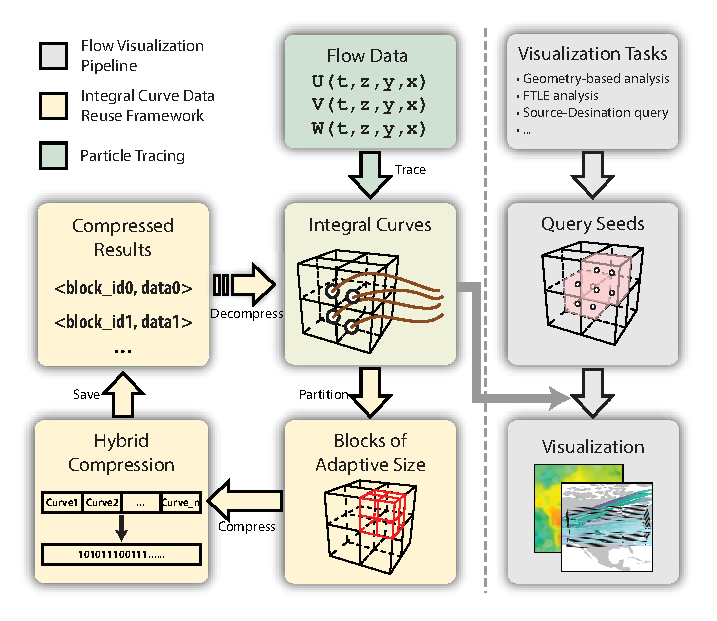
\includegraphics[width=.7\columnwidth]{image/linecompress/workflow.eps}
	\caption{
	基于压缩的积分曲线重用框架的流程\parencite{hong2017compression}。
	}
	\label{fig:workflow}
\end{figure}

基于压缩的积分曲线重用框架的可视化流程如图所示。该框架主要包括两部分:压缩和解压缩部分。前一部分只对一个数据集运行一次,采用稠密种子进行对整个流场进行数值积分,然后压缩曲线,并将结果保存到存储结构中。为了减少计算时间,该过程可以在大型计算集群中运行以大大降低处理时间。在运行一次之后,解压缩的模块可以为大型流场计算提供有力的支持,对于该部分的处理算法,同样支持并行计算。

积分曲线压缩是该工作中实现数据重用目标的核心技术,其主要障碍来自大体量中间数据。针对这一计算过程,该工作确定了三个优化目标。

{\bf 高压缩比}\quad
粒子追踪通常需要数百或数千个积分步骤才能生成种子的积分曲线,如果算法将种子放置在每个网格点上,则积分曲线的大小将比原始流场大数百倍或数千倍。在该方法提供的压缩方案中,存储非常需要高压缩比。在以下部分中,该工作使用压缩率进行比较。

{\bf 可控的信息丢失}\quad
压缩算法通常以牺牲数据的精确度为代价来实现高压缩率。信息丢失率低,可以确保可视化结果中不会有太多不确定性。对于各种数据集和可视化任务,最终用户对积分曲线的信息损失可能具有不同的容忍度。该工作希望提供某种机制来帮助控制不同情况下的信息丢失。

{\bf 快速检索}\quad
该工作采用基于压缩的重用框架的目的是使用高效的积分曲线提供程序来替换昂贵的粒子跟踪过程。快速检索是加速可视化应用程序的关键因素。大大降低的检索成本也是该工作对重用框架的主要贡献。

\begin{figure}[htbp]
  \centering
  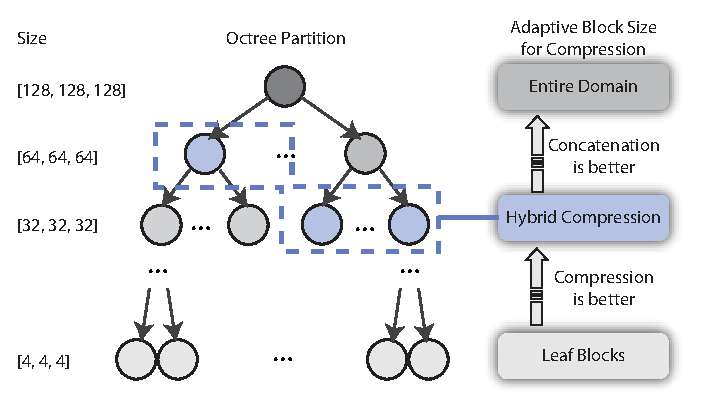
\includegraphics[width=.75\columnwidth]{image/linecompress/recursion.eps}
  \caption{
  基于八叉树空间划分的自适应大小块压缩算法\parencite{hong2017compression}。
  }
  \label{fig:recursion}
\end{figure}

为了平衡上述三个目标,设计了分层和混合压缩方案。具体地,将单独的曲线压缩方法和曲线组压缩方法组合以实现高压缩比并且保持低信息损失。在当前的实现中,该方法分别选择Bezier曲线拟合和fpzip方法。该方法通过将混合压缩方法应用于八叉树划分上的自适应大小的块,以平衡解压缩成本和压缩率。作为一种一般的计算框架,其他压缩算法同样可以代替该实现中的算法,只要在其他压缩算法可以满足上述的目标。

上述的混合压缩仅考虑压缩率与信息丢失之间的权衡。而对于某些方法,例如fpzip库,压缩率和解压缩成本都与块大小高度相关。为了平衡压缩率和解压缩成本,该工作采用八叉树结构将域分层划分为自适应块大小,以进行混合压缩。八叉树空间划分的一种常见用法,其基于某种度量在3D空间中选择合适的细节级别。在该工作框架中,算法自适应地选择更好的块大小以沿八叉树结构进行压缩。具体而言,对于八叉树结构中的一个节点,例如一个种子块,该方法有两种方法来压缩其相应的积分曲线。一种方法是直接应用混合压缩,这有望充分利用所有曲线的空间相干性来获得高压缩率。另一种方法是将其8个子节点(子块)的压缩结果串联为当前块的压缩结果。当仅仅需要稀疏的积分曲线时该方案可以避免解压缩,十分有效。在对每个节点进行选择之后,该工作实际上压缩了多个不同大小的块(蓝色)。对于这些块,该工作将其标识和相应的压缩结果存储在持久存储中以备将来使用。算法的具体流程如图所示。对于上述两种方式的选取,该方法在不同的阈值上进行了多次实验,测量了总压缩比和总解压缩成本。该方式根据经验可以选择了一个阈值,来达成这两种方式优劣的平衡。

\subsection{小结}
该小节综述了大规模科学数据中数据约减的已有核心工作和研究趋势,并以流场可视化中基于压缩的积分曲线重用框架工作为例,详细剖析了数据约减应对可视化或可视分析大规模科学数据流程的挑战的有效性。数据约减策略通过关注大规模数据中的共有趋势或特征,将数据的表示方式加以更变,创造出高效的数据结构和表达形式,以适应可视化和可视分析流程,可以十分有效地减少计算的开销,提升分析和计算结果反馈的实时性,是大规模科学数据管理中重要的组成部分。


